%------------------------------------------------
\begin{frame}
 \frametitle{Implementation of fast switches\footnote{developed together with Fa.\ barthel HF-Technik GmbH, Aachen} at RF Wien filter}	
 \framesubtitle{Modification of driving circuit\,\textcolor{PineGreen}{\cite{Slim:2020ufk}}}
 
\vspace{-0.3cm}  
\begin{center}
 	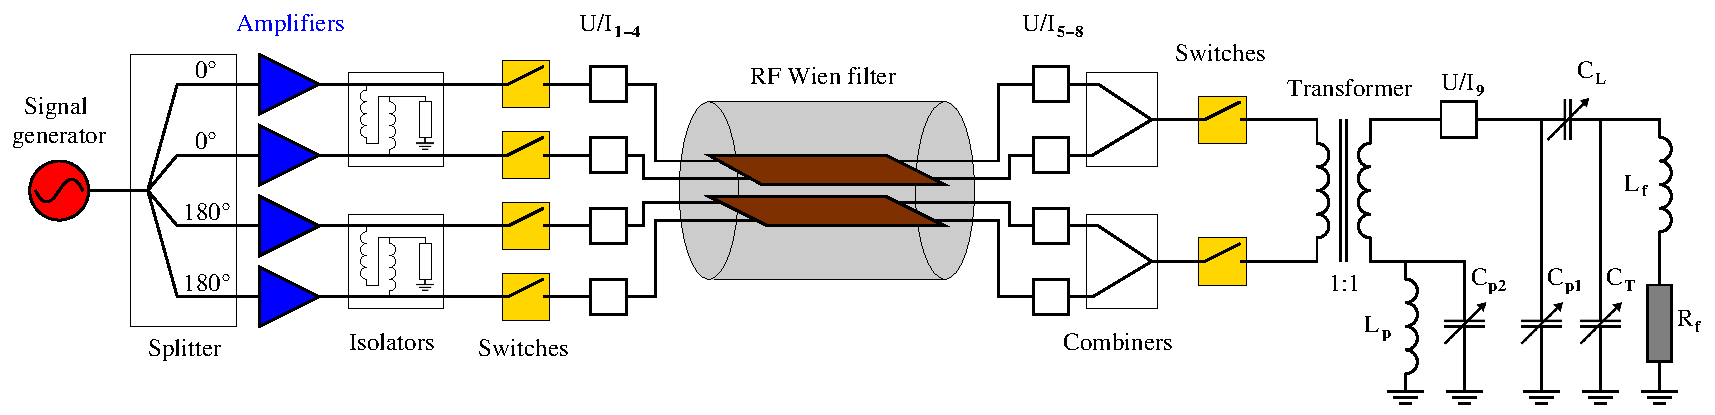
\includegraphics[width = 1\textwidth]{drivingcircuit-switches-1.pdf}
\end{center}
 
\vspace{-0.3cm} 
\begin{columns}
 \column{0.6\textwidth}
\begin{small}
\textbf{GaN HEM FET-based solution:}
 \begin{itemize}
    \item Short switch on/off times ($\approx$ few ns).
    \item High power capabilities ($\approx$ few kV).
    \item On board power damping ($-\SI{30}{\decibel}$ ).
    \item Symmetric switch on/off times ($\approx$ few ns).
  \end{itemize}
\end{small}
 
\column{0.35\textwidth}
\begin{center}
  \includegraphics<1>[height = 0.6\textwidth]{fast-switch}
  \includegraphics<2>[height = 0.6\textwidth]{gating_15052023.pdf}
  \end{center}
\end{columns}

\begin{alertblock}{Switches}
\begin{itemize}
 \item capable to handle up to \SI{200}{W} each
 \item permits system to run near a total power of \SI{0.8}{kW} in pulsed mode
\end{itemize}
\end{alertblock}
  
\end{frame}
%------------------------------------------------
